%%%%%%%%%%%%%%%%%%%%%%%%%%%%%%%%%%%%%%%%%%%%%%%%%%%%%%%%%%%%%%%%%%%%%%%%%%%%
% AGUJournalTemplate.tex: this template file is for articles formatted with LaTeX
%
% This file includes commands and instructions
% given in the order necessary to produce a final output that will
% satisfy AGU requirements, including customized APA reference formatting.
%
% You may copy this file and give it your
% article name, and enter your text.
%
% Step 1: Set the \documentclass

%% To submit your paper:
\documentclass[draft]{agujournal2019}
\usepackage{url} %this package should fix any errors with URLs in refs.
\usepackage{lineno}
\usepackage[inline]{trackchanges} %for better track changes. finalnew option will compile document with changes incorporated.
\usepackage{soul}
\usepackage{graphicx}

\usepackage{textgreek}
\usepackage[greek,english]{babel}
\usepackage{upgreek}
\usepackage{subcaption}
\usepackage{adjustbox}
\usepackage{multirow}

\usepackage[final]{listings}
\usepackage{xcolor}
\definecolor{codeblue}{RGB}{19, 0, 255}
\definecolor{codegreen}{RGB}{0, 129, 0}
\definecolor{codegray}{rgb}{0.5,0.5,0.5}
\definecolor{codered}{RGB}{163, 21, 21}
\definecolor{backcolour}{rgb}{0.95,0.95,0.92}

\lstdefinestyle{mystyle}{
    backgroundcolor=\color{backcolour},
    commentstyle=\color{codegreen}, 
    keywordstyle=\color{codeblue}, 
    numberstyle=\tiny\color{codegray}, 
    stringstyle=\color{codered},
    basicstyle=\footnotesize, 
    columns=flexible,
    breakatwhitespace=false,         
    breaklines=true,                 
    captionpos=b,                    
    keepspaces=true,                 
    numbers=left,                    
    numbersep=8pt,                  
    showspaces=false,                
    showstringspaces=false,
    showtabs=false,                  
    tabsize=3}
\lstset{style=mystyle}

\linenumbers
%%%%%%%
% As of 2018 we recommend use of the TrackChanges package to mark revisions.
% The trackchanges package adds five new LaTeX commands:
%
%  \note[editor]{The note}
%  \annote[editor]{Text to annotate}{The note}
%  \add[editor]{Text to add}
%  \remove[editor]{Text to remove}
%  \change[editor]{Text to remove}{Text to add}
%
% complete documentation is here: http://trackchanges.sourceforge.net/
%%%%%%%
\draftfalse

%% Enter journal name below.
%% Choose from this list of Journals:
% JGR: Atmospheres; JGR: Biogeosciences; JGR: Earth Surface; JGR: Oceans; JGR: Planets; JGR: Solid Earth
% Geophysical Research Letters; Reviews of Geophysics; Tectonics
% Geochemistry, Geophysics, Geosystems
% ie, \journalname{Water Resources Research}

\journalname{Default: Geochemistry, Geophysics, Geosystems}

\begin{document}

\graphicspath{{Figures/}}

%% ------------------------------------------------------------------------ %%
%  Title
% (A title should be specific, informative, and brief. Use
% abbreviations only if they are defined in the abstract. Titles that
% start with general keywords then specific terms are optimized in
% searches)
\title{PyBaselines: An Open-Source MCMC Algorithm for Fitting Baselines to FTIR Spectra of Basaltic-Rhyolitic Glasses}
%% ------------------------------------------------------------------------ %%
%% ------------------------------------------------------------------------ %%
%
%  AUTHORS AND AFFILIATIONS
%
%% ------------------------------------------------------------------------ %%

% Authors are individuals who have significantly contributed to the
% research and preparation of the article. Group authors are allowed, if
% each author in the group is separately identified in an appendix.)

% List authors by first name or initial followed by last name and
% separated by commas. Use \affil{} to number affiliations, and
% \thanks{} for author notes.
% Additional author notes should be indicated with \thanks{} (for
% example, for current addresses).

% Example: \authors{A. B. Author\affil{1}\thanks{Current address, Antartica}, B. C. Author\affil{2,3}, and D. E.
% Author\affil{3,4}\thanks{Also funded by Monsanto.}}

\authors{Alphabetical Ordering for Now: Anna Barth\affil{1, 2}, Terry Plank\affil{1}, Dan Rasmussen\affil{1, 3}, Sarah Shi\affil{1, 4}, Henry Towbin\affil{1}}

\affiliation{1}{Lamont-Doherty Earth Observatory, Columbia University. New York, NY USA}
\affiliation{2}{University of California, Berkeley. Berkeley, CA USA}
\affiliation{3}{National Museum of Natural History, Smithsonian Institution. Washington, DC USA}
\affiliation{4}{University of Cambridge ? Necessary, I don't know.}
%(repeat as many times as is necessary)

%% Corresponding Author:
% Corresponding author mailing address and e-mail address:

% (include name and email addresses of the corresponding author.  More
% than one corresponding author is allowed in this LaTeX file and for
% publication; but only one corresponding author is allowed in our
% editorial system.)

% Example: \correspondingauthor{First and Last Name}{email@address.edu}
\correspondingauthor{Sarah Shi}{scs2202@columbia.edu}
\correspondingauthor{Henry Towbin}{wht2106@columbia.edu}

%% Keypoints, final entry on title page.
%  List up to three key points (at least one is required)
%  Key Points summarize the main points and conclusions of the article
%  Each must be 140 characters or fewer with no special characters or punctuation and must be complete sentences

% Example:
% \begin{keypoints}
% \item	List up to three key points (at least one is required)
% \item	Key Points summarize the main points and conclusions of the article
% \item	Each must be 140 characters or fewer with no special characters or punctuation and must be complete sentences
% \end{keypoints}

\begin{keypoints}
\item 1
\item 2
\end{keypoints}

%% ------------------------------------------------------------------------ %%
%  ABSTRACT and PLAIN LANGUAGE SUMMARY
% A good Abstract will begin with a short description of the problem
% being addressed, briefly describe the new data or analyses, then
% briefly states the main conclusion(s) and how they are supported and
% uncertainties.

% The Plain Language Summary should be written for a broad audience,
% including journalists and the science-interested public, that will not have 
% a background in your field.
%
% A Plain Language Summary is required in GRL, JGR: Planets, JGR: Biogeosciences,
% JGR: Oceans, G-Cubed, Reviews of Geophysics, and JAMES.
% see http://sharingscience.agu.org/creating-plain-language-summary/)
%
%% ------------------------------------------------------------------------ %%

%% \begin{abstract} starts the second page

\begin{abstract}


\end{abstract}

%\section*{Plain Language Summary}
%[ enter your Plain Language Summary here or delete this section]


%% ------------------------------------------------------------------------ %%
%
%  TEXT
%
%% ------------------------------------------------------------------------ %%

%%% Suggested section heads:
% \section{Introduction}
%
% The main text should start with an introduction. Except for short
% manuscripts (such as comments and replies), the text should be divided
% into sections, each with its own heading.

% Headings should be sentence fragments and do not begin with a
% lowercase letter or number. Examples of good headings are:

% \section{Materials and Methods}
% Here is text on Materials and Methods.
%
% \subsection{A descriptive heading about methods}
% More about Methods.
%
% \section{Data} (Or section title might be a descriptive heading about data)
%
% \section{Results} (Or section title might be a descriptive heading about the
% results)
%
% \section{Conclusions}

\section{Introduction} % Section
The variability and subjectivity in Fourier Transform Infrared Spectroscopy (FTIR) baseline fitting techniques constitutes a major uncertainty in the determination of volatile concentrations. We develop quantifiable and reproducible approaches to defining baselines beneath each H$_{2}$O and CO$_2$ species peak to determine concentrations with meaningful uncertainties, unlike most FTIR studies, where baselines are fit by eye, spline, instrument software, or unspecified means. 


The \textepsilon$_{\mathrm{H_2O_{t, 3550}}}$ peak can be well quantified with a linear to near-linear baseline between the two absorbance minima on either side of peak when the peak is unsaturated with a raw absorbance of \textless 2 ~\cite{DixonandStolper1995, vonAulocketal2014}. When \textepsilon$_{\mathrm{H_2O_{t, 3550}}}$ is saturated, the combination of H$_{2}$O$_{\mathrm{m}, 5200}$ or the H$_{2}$O$_{\mathrm{m}, 1635}$ and the OH$^{-}_{4500}$ must be used instead. The H$_{2}$O$_{\mathrm{m}, 5200}$ and OH$^{-}_{4500}$ peaks can be fit with a linear to near-linear baseline, or a baseline consisting of two Gaussians~\cite{Ohlhorstetal2001, Stabileetal2020, Stolper1982, WithersandBehrens1999}. The linear to near-linear baseline is advantageous given the reproducibility of peak heights but can underestimate the peak height or area given the presence of iron and water-related bands ($\sim$5700 and $\sim$4000 cm$^{-1}$, respectively) in dacitic to basaltic compositions~\cite{Ohlhorstetal2001}. The species concentration of H$_{2}$O$_{\mathrm{m}, 5200}$ and OH$^{-}_{4500}$ by the two Gaussian method agrees well with NMR spectroscopy but is highly sensitive to raw absorbance and can be difficult to reproduce across studies~\cite{Ohlhorstetal2001}. The \textepsilon$_{\mathrm{H_2O_{t, 3550}}}$, H$_{2}$O$_{\mathrm{m}, 5200}$, and OH$^{-}_{4500}$ baselines are thus fit with the asymmetric least squares (ALS) method, iteratively solving for an interpolated fitting which balances smoothness and asymmetry~\cite{Eilers2004, Leeetal2017, Pengetal2010}

The H$_{2}$O$_{\mathrm{m}, 1635}$ peak and CO$_{3}^{2-}$ doublet peaks pose greater challenges due to the steep and sharp increase of baseline absorbance at wavenumbers lower than 1430 cm$^{-1}$. Furthermore, the convolution of the tails of the H$_{2}$O$_{\mathrm{m}, 1635}$ and the CO$_{3}^{2-}$1515 doublet peak in melt inclusion spectra further complicates the appropriate baselines in the near infrared region. Baselines beneath the H$_{2}$O$_{\mathrm{m}, 1635}$ and CO$_{3}^{2-}$ doublet peaks have been approximated with the spectra of devolatilized samples with similar chemical compositions~\cite{Dixonetal1988, Newmanetal2000}, splines and flexicurves~\cite{DixonandStolper1995}, and other curve functions~\cite{DixonandClague2001}. We assess the fundamental shape and variability of the baseline using principal component analysis (PCA) applied to a database of absorbance spectra for volatile-poor melt inclusions from the Aleutian arc~\cite{RasmussenThesis} and MORB glasses~\cite{Newmanetal2000}. This dataset of naturally devolatilized spectra is relevant to a wide range of arc and MORB compositions. The application of PCA to a training dataset of devolatilized spectra allows for the assessment of the fundamental shape of the baseline and the spectral features contributing to variability~\cite{Carvajaletal2016}. We develop and present a method for fitting baselines and peaks with uncertainties for the H$_{2}$OT, H$_{2}$O$_{\mathrm{m}, 5200}$, and OH$^{-}_{4500}$ peaks with repeat asymmetric least squares baselines and the H$_{2}$O$_{\mathrm{m}, 1635}$ peak and the CO$_{3}^{2-}$ doublet peaks with Bayesian statistics and a Python Multi-Core Markov Chain Monte Carlo algorithm. 

\section{Analytical Methodology} % Section - 1.4
\subsection{Transmission Fourier Transform Infrared Spectroscopy (FTIR)}
Natural glass standards and olivine-hosted melt inclusions (MIs) were analyzed with the Thermo Scientific Nicolet iN10 MX Fourier Transform Infrared (FTIR) Spectrometer at the Lamont-Doherty Earth Observatory. Transmission FTIR spectroscopy measures the amount of light absorbed at each wavelength, allowing for the recognition and quantification of volatile species with the Beer-Lambert Law: 
\begin{equation}
c = \frac{A M}{\varepsilon l \rho}
\end{equation}
where $c$ is concentration, $A$ is absorbance, $M$ is the molar mass of the absorbing volatile species (g$\cdot$mol$^{-1}$), \textepsilon{} is the absorptivity of the species (L$\cdot$mol$^{-1}\cdot$ cm), $l$ is the optical path length or thickness (cm), and \textrho{} is density (kg$\cdot$m$^{-3}$). Linear relationships between absorbance and concentration dominate. Non-linear relationships can be introduced when increased sample thicknesses result in insufficient light transmission to the detector, pushing peaks to become saturated as with ${\mathrm{H_2O_{t, 3550}}}$~\cite{McIntoshetal2017, vonAulocketal2014}. 

Glass standards and MIs were placed on a CaF$_2$ plate within the sample holder for measurement of IR absorbance during transmission in the detector spectral range of 8000-450 wavenumbers (cm$^{-1}$). The FTIR was purged for twenty minutes to decrease the signal of atmospheric H$_{2}$O and CO$_{2}$. Glasses and MIs were mapped for absorbance to determine potential heterogeneity in volatile concentrations and to determine the boundaries of measurement — particularly for MI to ensure double intersection. Absorbance maps were generated at a point spacing of 10$\times$10 \textmu m, with 16 scans taken at each point at a resolution of 16 cm$^{-1}$. The relatively few scans and low resolution were balanced to yield manageable mapping times of approximately 15 minutes for each MI. Maps guided the selection of optimal regions for volatile analyses. Three repeat measurements were collected for each glass standard or MI, with 256 collection scans at 4 cm$^{-1}$ spectral resolution. Background scans were collected under the same conditions through the CaF$_{2}$ plate. Aperture sizes (30-200 \textmu m for glass standards and 15-50 \textmu m for MIs) were selected to maximize analytical area and to ensure that light propagated solely through the MI without including the host olivine. The Happ-Genzel apodization function within the Thermo-Nicolet OMNIC Picta software was applied to each spectrum to maintain resolution and reduce noise. Three repeat measurements were taken for each MI. Internal standards of submarine arc lava GH88-1-D1010 analyzed by~\citeA{Newmanetal2000} with FTIR and basaltic MIs CN\_C\_OL1’, CN92C\_OL2, and ETF46 analyzed by~\citeA{Barthetal2019} and~\citeA{BarthThesis} with SIMS were measured at the beginning and end of each analytical session as internal check standards. 

\subsection{Reflectance Fourier Transform Infrared Spectroscopy (FTIR)}
Three repeat thickness measurements of olivine-hosted melt inclusions were acquired using a Mitutoyo 543-783B Digimatic Indicator, as well as with the reflectance method described by~\citeA{NicholsandWysoczanski2007}. Wavelengths of interference fringes are proportional to the thickness and refractive index of the sample for thin silica films~\cite{Nishikidaetal1996, Tamicetal2001, WysoczanskiandTani2006, Sunetal2007}.~\citeA{Nishikidaetal1996} show the relationship applicable to glasses and olivine: 
\begin{equation}
l = \frac{m}{2n (v_1 - v_2)}
\end{equation}
where $l$ is the thickness of area analyzed, $m$ is the number of fringes in the wavenumber range, $n$ is the refractive index of the material, and $v_1$ and $v_2$ are the highest and lowest wavenumbers in the interval. Interference fringes are produced by the interactions between reflected light and reflections internal to the sample, with fringe wavelengths inversely proportional to thickness. Two reflectance spectra were taken adjacent to olivine-hosted melt inclusions with 256 collection scans at 4 cm$^{-1}$ spectral resolution, with aperture sizes of 50$\times$50 \textmu m. Background scans were collected under the same conditions on a highly reflective gold plate with a reflectance coefficient of unity~\cite{NicholsandWysoczanski2007}. The basaltic glass refractive index is quantified to be 1.546~\cite{KumagaiandKaneoka2003}. The rhyolitic glass refractive index is not as well quantified, showing additional variability and spanning the range of 1.48\textless $n$\textless 1.51~\cite{Trogeretal1959, Tamicetal2001}. Refractive indices for glasses of variable composition can be calibrated with the digital micrometer~\cite{DuncanandDasgupta2015, Tamicetal2001}. The olivine mean refractive index, averaged across the three crystallographic axes, is described by forsterite content with linear relationships described in~\citeA{DHZ1992}. 

\subsection{Electron Probe Microanalyzer (EPMA)}
Major and trace elements in glass and olivine were analyzed by wavelength dispersive X-ray spectroscopy with the Cameca SXFive-TACTIS electron microprobe (EPMA) at the American Museum of Natural History. Calibration was completed with natural and synthetic mineral and oxide standards. Glasses were measured with an accelerating voltage of 15 keV, variable working current of 4 nA, 10 nA, and 40 nA, and spot size of 10 \textmu m. Duplicate MI analyses were collected proximal to the center of the inclusion. Na was measured with a working current of 4 nA with 2 s counting on peak and 20 s on background to minimize Na loss. Other major and trace elements were measured with a working current of 10 nA with 30 s counting on peak and 15 s on background. Fe was analyzed with 20 s counting on peak and 15 s on background. Volatiles S and Cl were measured with an increased working current of 40 nA. Olivines were measured with an accelerating voltage of 15 keV, variable working current of 10 nA and 300 nA, and spot size of 1 \textmu m. Duplicate olivine-host analyses were collected approximately 15 \textmu m from the MI. Mg, Si, and Fe were analyzed with a working current of 10 nA, and all remaining minor and trace elements were analyzed with a working current of 300 nA. \textbf{I can't figure out all the counting times from the files, need a bit of help with this for appendix}. Replicate analyses of the check standard MR:ND-70-01 and secondary standards San Carlos Olivine and VG-2 were performed every 10 analyses. Column conditions and additional assessments of Instrumental drift, precision, and accuracy from analysis of standard analyses are provided in~\ref{supplement:a}. 

%Relative proportions of oxidized and reduced S impacts the S valence state and bond energies, which in turn shifts the wavelength of SK\textalpha-radiation~\cite{CarrollandRutherford1988, WallaceandCarmichael1994}. The S peak position was initially calibrated at the peak position for S$^{6+}$, at 61435 sin\straighttheta, using a standard BaSO$_{4}$. The other endmember position for S$^{2-}$ was calibrated with two basaltic check standards, VG-2 and MR-ND-70-01, at 61470 sin\straighttheta \ (Supplement~\ref{supplement:a}). Several wavescans of Fuego melt inclusions were taken to assess the oxidation state and to determine the appropriate peak position on which to measure S. The Fuego melt inclusion wavescans had near-identical peak locations at 61370 sin\straighttheta{}, indicating that the S peak had shifted towards BaSO$_{4}$ (Supplement~\ref{supplement:a}). The peak position was set at 61370 sin\straighttheta{} to measure all melt inclusions. 

\section{PyBaselines Structure and Computational Methodology} % Section - 1.4
\subsection{PyBaselines Structure}
PyBaselines can be locally installed with Python versions $\ge$ 3.6 using the command line: 
\begin{lstlisting}[language=Python]
pip install PyBaselines 
\end{lstlisting}
and installed with Google Colab and Binder, two cloud-based Python development environments, where installation occurs within a code cell: 
\begin{lstlisting}[language=Python]
!pip install PyBaselines 
\end{lstlisting}
The PyBaselines package must then be loaded and initialized with: 
\begin{lstlisting}[language=Python]
import PyBaselines as bl
\end{lstlisting}
Functions from PyBaselines are then called with the abbreviated package name, followed by a dot, followed by the function name. The function loading all spectrum files is called as follows: 
\begin{lstlisting}[language=Python]
bl.Load_SampleCSV(args)
\end{lstlisting}
and the function processing each spectrum file is called as follows: 
\begin{lstlisting}[language=Python]
bl.Run_All_Spectra(args)
\end{lstlisting}

\subsection{Calculating Thickness from Reflectance FTIR Spectra}
We develop an automated implementation for calculating thicknesses from reflectance spectra by the interference fringe method with the function: 
\begin{lstlisting}[language=Python]
bl.ThicknessProcessing(dfs_dict, n, wn_high, wn_low, peak_height_min_delta, peak_search_width)
\end{lstlisting}
Signal-to-noise ratios associated with interference fringes can be low. Reflectance spectra are preprocessed with median filtering to remove potential single spike noise and successively processed with Savitzky-Golay filtering, fitting low-degree polynomials to data with linear least squares~\cite{SavitzkyandGolay1964}. Local extrema associated with each interference fringe wave are located by identifying regions of greatest absorbance change. Maxima are surrounded by points that are lower in absorbance and minima are surrounded by points that are greater in absorbance. Local extrema identification by differentiation can fail with noisier spectra. Thicknesses are calculated from the wavenumber differences between each sequential grouping of local maxima or minima within the inputted wavenumber range. 

Mean thicknesses and standard deviations from local maxima and minima are determined and compared against those from digital micrometer to assess the uncertainty associated with this method. Two to eight interference fringes in the wavenumber range of 1700 to 2850 cm$^{-1}$ for Volcán de Fuego olivines. A refractive index 


was determined with the average Fo$_{72}$ composition for spots adjacent to melt inclusions using the linear relationships d

Increasing the wavenumber range compared to that of~\citeA{NicholsandWysoczanski2007} increases the number of high-quality interference fringe waves while reproducing digital micrometer measurements. Average thickness uncertainties associated with five measurements is similar to previously reported values at less than 3 \textmu m~\cite{Allisonetal2019, NicholsandWysoczanski2007, vonAulocketal2014}. Thickness by the reflectance fringe method was uniformly greater than that by the digital micrometer, likely suggesting that the olivine refractive index calculated from~\citeA{DHZ1992} is too low. Uncertainties in the refractive index may exist, given the lack of parameterization of composition dependence and the lack of recent analyses.


\subsection{Calibrating Molar Absorptivity (\textepsilon)}
Molar absorptivities or extinction coefficients (\textepsilon) determine the intensity at which light attenuates when passing through a material and relates absorbance to concentration, calibrated by pairing analyses of volatile content by transmission FTIR and by an additional independent analytical technique. \textepsilon is dependent on the composition of glass, related to both tetrahedral cation fraction of $\uptau$=(Si$^{4+}$+Al$^{3+}$)/(total cations) and cation fraction of Na$^{+}$/(Na$^{+}$+Ca$^{2+}$). We refit these extinction coefficients to incorporate all quantifications of extinction coefficients since the last compilation of extinction coefficients by~\citeA{Mandevilleetal2002}.

The extinction coefficients related to H$_2$O species increase with tetrahedral cation fraction, $\uptau$, reflecting increased polymerization of the glass~\cite{Stolper1982}. Tetrahedral cations have also been proposed to compete with non-tetrahedral cations (M = Mg$^{2+}$, Ca$^{2+}$, Na$^{+}$) to bond with free hydroxyl groups in melt~\cite{Mercieretal2010, Pandyaetal1992}. More depolymerized melts will have higher proportions of free hydroxyl, which translates to more M-(OH)$_x$ bonding and hydrogen bonding~\cite{Mercieretal2010, Xue2009}.~\citeA{Dixonetal1995} and~\citeA{Mandevilleetal2002} demonstrate the dependence of the \textepsilon${\mathrm{H_2O_{m, 5200}}}$, \textepsilon${\mathrm{OH^{-}_{4500}}}$, and \textepsilon${\mathrm{H_2O_{m, 1635}}}$ on glass tetrahedral cation fraction. Tetrahedral cation fraction is similarly observed to be positively correlated with \textepsilon$_{\mathrm{H_2O_{t, 3550}}}$, but this relationship is less straightforward~\cite{Mercieretal2010}. Quench temperatures and rates will drive the formation of variable proportions of H$_{2}$O$_{\mathrm{m}}$ and OH$^{-}$~\cite{SilverandStolper1989, Stolper1989}. \textepsilon$_{\mathrm{H_2O_{t, 3550}}}$ has thus been considered as a combination of two endmember absorption coefficients, \textepsilon$_{\mathrm{OH^{-}_{3550}}}$ and \textepsilon$_{\mathrm{H_2O_{m, 3550}}}$, multiplied by the relative proportion of each respective species~\cite{McIntoshetal2017, Newmanetal1986, Okumuraetal2003}. Studies quantifying \textepsilon$_{\mathrm{OH^{-}_{3550}}}$ and \textepsilon$_{\mathrm{H_2O_{m, 3550}}}$ are the gold standard, but are currently limited in compositional range;~\citeA{McIntoshetal2017} considered the range of $\uptau$ = 0.746-0.800, spanning silicic compositions from rhyolitic to albitic glasses. More experiments are needed to properly quantify the species-dependent nature of the $\mathrm{H_2O_{t, 3550}}$ peak. 

~\citeA{DixonandPan1995} first demonstrate the dependence of the CO$_{3}^{2-}$ doublet absorption coefficients on the molar or cationic ratio of Na$^{+}$/(Na$^{+}$+Ca$^{2+}$). The proportion of Na$^{+}$ to Ca$^{2+}$ modulates the dissolution of C as molecular CO$_{2}$ and/or CO$_{3}^{2-}$. As the proportion of Ca$^{2+}$ increases, \textepsilon$_{\mathrm{CO_3^{2-}}}$ decreases. C dissolves as both molecular CO$_{2}$ and CO$_{3}^{2-}$ in NaAl-rich silicate glasses (albitic, jadeitic, nephelinitic compositions)~\cite{DixonandPan1995, FineandStolper1985, MysenandVirgo1980a, MysenandVirgo1980b}. C solely dissolves as CO$_{3}^{2-}$ in Ca and CaMg-rich silicate glasses (diopsidic, sodamelilitic, and akermanitic compositions)~\cite{DixonandPan1995, FineandStolper1986}.

We refit the linear relationships between \textepsilon$_{\mathrm{CO_3^{2-}}}$, \textepsilon$_{\mathrm{OH^{-}_{4500}}}$, \textepsilon$_{\mathrm{H_2O_{t, 3550}}}$, \textepsilon$_{\mathrm{H_2O_{m, 1635}}}$, and \textepsilon$_{\mathrm{CO_3^{2-}}}$ and the corresponding compositional parameters of $\uptau$ or Na$^{+}$/(Na$^{+}$+Ca$^{2+}$) values to include more recent data and broader compositional ranges, with an implicit inverse method based on that described in Chapter 9 of~\citeA{Menke2018}. 


Uncertainties in \textepsilon, due to variability in independent volatile measurements, and compositional parameters, related to older microprobe measurements with incomplete oxide measurements, can thus be accounted for within the model. The \textepsilon data are limited to studies with independent methods of volatile measurement – such as SIMS, Karl Fischer titration, experimental mass balance, vacuum heating, or manometry – and with H$_{2}$O $>$ 0.5 wt.\% for peak resolution. In the full dataset, $\uptau$ spans the range of 0.50-0.90 and Na$^{+}$/(Na$^{+}$+Ca$^{2+}$) from 0.23-0.84, encompassing that for the Fuego 2018 MIs ($\uptau$ = 0.66-0.71 and Na$^{+}$/(Na$^{+}$+Ca$^{2+}$) = 0.39-0.56). If \textepsilon$_{\mathrm{CO_3^{2-}}}$ or \textepsilon$_{\mathrm{OH^{-}_{4500}}}$ are quantified with both a linear and two Gaussian baseline, we average the two estimates. Although not typically quantified, we find a positive relationship between \textepsilon$_{\mathrm{H_2O_{t, 3550}}}$ and $\uptau$, despite complications presented by the speciation (Supplemental Figure xx). The relationship observed with NBO/T, calculated by methods outlined in~\citeA{MysenandRichet2018}, is not observed in this dataset, despite the observation in~\citeA{Mercieretal2010} (Supplemental Figure xx). 

While endmember data for H$_{2}$O$_{\mathrm{t, 3550}}$ remain limited, \textepsilon$_{\mathrm{H_2O_{t, 3550}}}$ is best fit with $\uptau$. \textepsilon$_{\mathrm{CO_3^{2-}}}$ data are often limited to either the \textepsilon$_{\mathrm{CO_{3, 1515}^{2-}}}$ or \textepsilon$_{\mathrm{CO_{3, 1430}^{2-}}}$ peak, which are also assumed to be approximately equal~\cite{DixonandPan1995}. A cumulative \textepsilon$_{\mathrm{CO_3^{2-}}}$ is fit with data from \textepsilon$_{\mathrm{CO_{3, 1515}^{2-}}}$ or \textepsilon$_{\mathrm{CO_{3, 1430}^{2-}}}$, where available, given the variability in the baseline fitting method. This regression is appropriate for the compositional range of calibration (Na$^{+}$/(Na$^{+}$+Ca$^{2+}$) = 0.23-0.84). The behavior of the absorption coefficient at the Na$^{+}$ and Ca$^{2+}$ endmembers is complex and these compositions are not considered in this study. An uncertainty of 10\% is applied to \textepsilon$_{\mathrm{CO_3^{2-}}}$, \textepsilon$_{\mathrm{H_2O_{t, 3550}}}$, \textepsilon$_{\mathrm{H_2O_{m, 1635}}}$, and \textepsilon$_{\mathrm{CO_3^{2-}}}$ peaks. An uncertainty of 20\% is applied to the fits with \textepsilon$_{\mathrm{OH^{-}_{4500}}}$ given the increased uncertainty on the contrasting linear and Gaussian baseline fits to the peak. Uncertainties in the extinction coefficient fit, in combination with those for the microprobe session, are propagated forward to the posterior covariance on model parameter coefficients. 

\begin{figure}[htb!] 
\centering
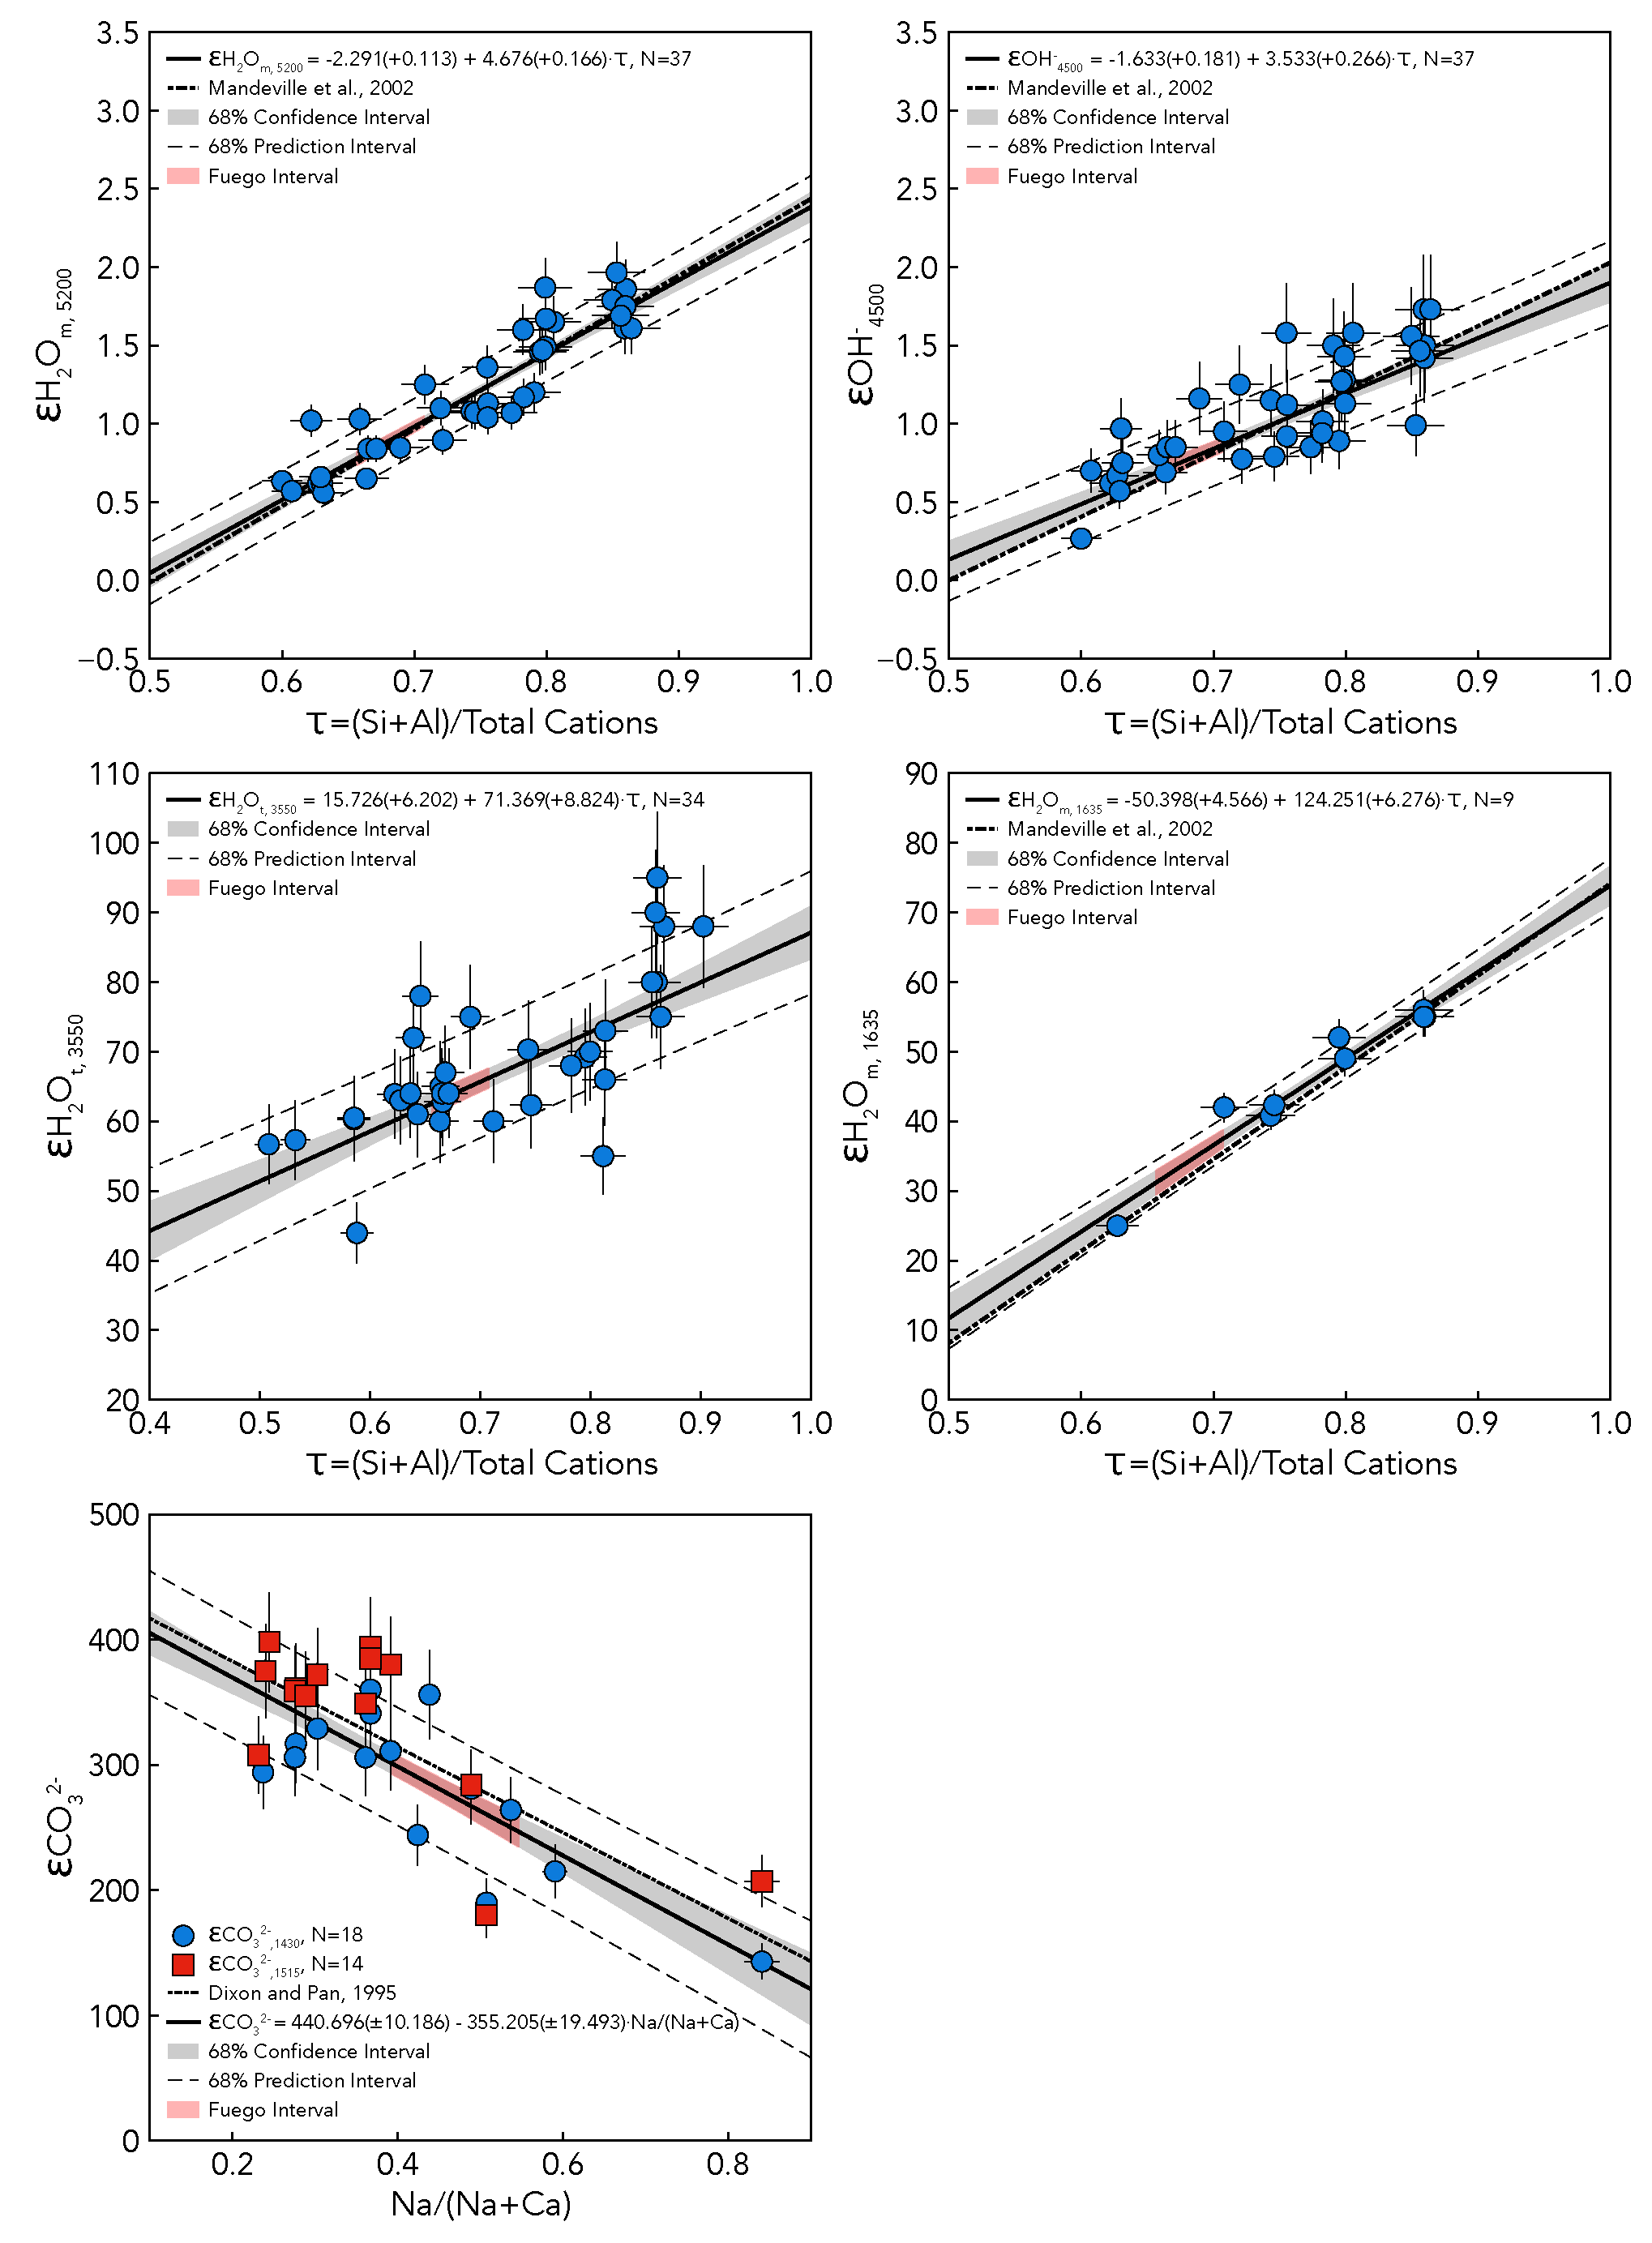
\includegraphics[width=1.0\textwidth]{AllEpsilonRegress}
\caption[Epsilon Regressions]{Epsilon regressions}
\label{figure:EpsilonRegressions}
\end{figure}


\subsection{Calculating Density}
Melt density is a function of the composition of the melt inclusion, and is calculated from the gram formula weight and partial molar volumes (at ambient temperature and pressure of the analytical conditions) from~\citeA{LesherandSpera2015}. The large molar volume of H$_{2}$O in arc basaltic melt inclusions strongly impacts density and requires the implementation of an iterative solver. The initial solution for density is assumed to have no contribution from H$_{2}$O but is updated with the calculated amount of H$_{2}$O$_{\mathrm{t, 3550}}$ or H$_{2}$O$_{\mathrm{m, 1635}}$ + OH$^{-}_{4500}$ if the sample is saturated. The density converges within 10 iterations. The final density, the appropriate absorption coefficient, and the ALS and MC$^3$ determined peak heights of absorbance are applied through the Beer Lambert Law to determine the concentration of H$_{2}$O$_{\mathrm{t}}$, H$_{2}$O$_{\mathrm{m}}$, OH$^{-}$, and CO$_{2}$ of each doublet peak. A standard deviation on each concentration is taken by running a simple Monte Carlo error assessment in which all parameters (except molar mass) are allowed to vary with a normal distribution for 5x10$^{5}$ samples.


\subsection{Assessing Baseline Variability}
\textbf{Henry's section}

\subsection{Monte Carlo Framework}

The net equation describing the absorbance spectrum of a glass or melt inclusion, with \textupsilon$^-$ defined as the wavenumber range from 2400 to 1275 cm$^{-1}$, is thus expressed in the following form:

where $x_{1}$, $x_{2}$, $x_{3}$, $y_{1}$, $y_{2}$, $a_{1515}$, $a_{1430}$, 1515, 1430, 1515, 1430, m, and b are the best fit parameters. These optimum fit parameters are first determined by ordinary least squares. The model parameter space of the modeled absorbance of the melt inclusion spectrum is sampled and explored by leveraging a Monte-Carlo Markov Chain algorithm in a Bayesian parametric framework, to account for uncertainty. In this framework of Bayesian inferences, the posterior joint probability distribution of model parameters is quantified as a function of the prior probability of model parameters and a likelihood function. Bayes’ Theorem dictates that the posterior joint probability distribution is updated as more information becomes available, following~\citeA{Cubillosetal2017}: 
\begin{equation}
P(\theta | y, M) \propto P(\theta | M) P(y | \theta, M),
\end{equation}
where $y$ denotes data, $\theta$ is the set of parameters, $P(\theta|y, M)$ is the posterior probability distribution of parameters, $P(\theta |M)$ is the prior probability distribution (not incorporating new information), and $P(y|\theta, M)$ is the likelihood. The prior probability distribution of parameters is defined by the expected range and distributions of these parameters. The likelihood serves as the probability density function of the modeled data given an array of parameters. A Markov-Chain Monte Carlo (MCMC) algorithm was utilized to generate random samples from the parameter space to generate and assess the parameter space, where the random samples generated by the algorithm hold a probability density distribution that is proportional to the posterior probability distribution. The open-source Python package, Multi-Core Markov-Chain Monte Carlo, or MC$^{3}$, integrates these statistical methods~\cite{Cubillosetal2017} and was implemented for this study.
Fixed absorbance spectra provide the information required to generate improved posterior probability distributions of model parameters. Prior probability distributions of the parameters generating the baseline, peaks, and lines require different functions – either uniform or Gaussian – to accurately represent this space. Parameters related to the baselines, molecular H$_{2}$O peak, CO$_{3}^{2-}$ doublet peak heights, and linear adjustment are sampled uniformly, given the greater variation within these parameters that is not defined around one value. The exploration space provided these uniformly sampled priors is guided by the initial model generation process. The CO$_{3}^{2-}$ doublet peak locations and standard deviations are defined with a Gaussian prior, given the well-defined nature of these parameters in basaltic melt inclusion absorbance spectra. The initial prior parameters are optimized with the least-squares Trust Region Reflective algorithm, which is suitable for well-constrained, large problems~\cite{Branchetal1999}. 

Random MCMC sampling is performed with the Snooker Updater Differential Evolution Markov Chain method (DEMC), which involves the parallel evolution of multiple chains and computation of appropriate scales and orientations for the jumping distribution~\cite{terBraak2006, terBraakandVrugt2008}. The scale and direction of the proposed jump is computed by the parallel computation of several chains, which allow for the differences between one chain and two additional randomly selected chains to evolve forwards. The chains will converge towards a posterior distribution and will align the evolution along the proper orientation, with good scaling. The Snooker Updater DEMC optimizes acceptance rates and efficiency, allowing for one melt inclusion spectrum to be run within 15 seconds. The Bayesian and MCMC framework underlying this model allows for numerous parameters to be sampled and fit concurrently, while credibly quantifying uncertainties. 



%  Numbered lines in equations:
%  To add line numbers to lines in equations,
%  \begin{linenomath*}
%  \begin{equation}
%  \end{equation}
%  \end{linenomath*}

%% Enter Figures and Tables near as possible to where they are first mentioned:
%
% DO NOT USE \psfrag or \subfigure commands.
%
% Figure captions go below the figure.
% Table titles go above tables;  other caption information
%  should be placed in last line of the table, using
% \multicolumn2l{$^a$ This is a table note.}
%
%----------------
% EXAMPLE FIGURES
%
% \begin{figure}
% \includegraphics{example.png}
% \caption{caption}
% \end{figure}
%
% Giving latex a width will help it to scale the figure properly. A simple trick is to use \textwidth. Try this if large figures run off the side of the page.
% \begin{figure}
% \noindent\includegraphics[width=\textwidth]{anothersample.png}
%\caption{caption}
%\label{pngfiguresample}
%\end{figure}
%
%
% If you get an error about an unknown bounding box, try specifying the width and height of the figure with the natwidth and natheight options. This is common when trying to add a PDF figure without pdflatex.
% \begin{figure}
% \noindent\includegraphics[natwidth=800px,natheight=600px]{samplefigure.pdf}
%\caption{caption}
%\label{pdffiguresample}
%\end{figure}
%
%
% PDFLatex does not seem to be able to process EPS figures. You may want to try the epstopdf package.
%

%
% ---------------
% EXAMPLE TABLE
%
% \begin{table}
% \caption{Time of the Transition Between Phase 1 and Phase 2$^{a}$}
% \centering
% \begin{tabular}{l c}
% \hline
%  Run  & Time (min)  \\
% \hline
%   $l1$  & 260   \\
%   $l2$  & 300   \\
%   $l3$  & 340   \\
%   $h1$  & 270   \\
%   $h2$  & 250   \\
%   $h3$  & 380   \\
%   $r1$  & 370   \\
%   $r2$  & 390   \\
% \hline
% \multicolumn{2}{l}{$^{a}$Footnote text here.}
% \end{tabular}
% \end{table}

%% SIDEWAYS FIGURE and TABLE
% AGU prefers the use of {sidewaystable} over {landscapetable} as it causes fewer problems.
%
% \begin{sidewaysfigure}
% \includegraphics[width=20pc]{figsamp}
% \caption{caption here}
% \label{newfig}
% \end{sidewaysfigure}
%
%  \begin{sidewaystable}
%  \caption{Caption here}
% \label{tab:signif_gap_clos}
%  \begin{tabular}{ccc}
% one&two&three\\
% four&five&six
%  \end{tabular}
%  \end{sidewaystable}

%% If using numbered lines, please surround equations with \begin{linenomath*}...\end{linenomath*}
%\begin{linenomath*}
%\begin{equation}
%y|{f} \sim g(m, \sigma),
%\end{equation}
%\end{linenomath*}

%%% End of body of article

%%%%%%%%%%%%%%%%%%%%%%%%%%%%%%%%
%% Optional Appendix goes here
%
% The \appendix command resets counters and redefines section heads
%
% After typing \appendix
%
%\section{Here Is Appendix Title}
% will show
% A: Here Is Appendix Title
%
%\appendix
%\section{Here is a sample appendix}

%%%%%%%%%%%%%%%%%%%%%%%%%%%%%%%%%%%%%%%%%%%%%%%%%%%%%%%%%%%%%%%%
%
% Optional Glossary, Notation or Acronym section goes here:
%
%%%%%%%%%%%%%%
% Glossary is only allowed in Reviews of Geophysics
%  \begin{glossary}
%  \term{Term}
%   Term Definition here
%  \term{Term}
%   Term Definition here
%  \term{Term}
%   Term Definition here
%  \end{glossary}

%
%%%%%%%%%%%%%%
% Acronyms
%   \begin{acronyms}
%   \acro{Acronym}
%   Definition here
%   \acro{EMOS}
%   Ensemble model output statistics
%   \acro{ECMWF}
%   Centre for Medium-Range Weather Forecasts
%   \end{acronyms}

%
%%%%%%%%%%%%%%
% Notation
%   \begin{notation}
%   \notation{$a+b$} Notation Definition here
%   \notation{$e=mc^2$}
%   Equation in German-born physicist Albert Einstein's theory of special
%  relativity that showed that the increased relativistic mass ($m$) of a
%  body comes from the energy of motion of the body—that is, its kinetic
%  energy ($E$)—divided by the speed of light squared ($c^2$).
%   \end{notation}

%%%%%%%%%%%%%%%%%%%%%%%%%%%%%%%%%%%%%%%%%%%%%%%%%%%%%%%%%%%%%%%%
% ACKNOWLEDGMENTS
% The acknowledgments must list:
% >>>>	A statement that indicates to the reader where the data
% 	supporting the conclusions can be obtained (for example, in the
% 	references, tables, supporting information, and other databases).
% 	All funding sources related to this work from all authors
% 	Any real or perceived financial conflicts of interests for any author
% 	Other affiliations for any author that may be perceived as
% 	having a conflict of interest with respect to the results of this paper.
% It is also the appropriate place to thank colleagues and other contributors.
% AGU does not normally allow dedications.


\acknowledgments
Enter acknowledgments, including your data availability statement, here.

%% ------------------------------------------------------------------------ %%
% SUPPLEMENT

\appendix
\section{Supplement: EPMA Analytical Conditions, Precision, and Accuracy}

\label{supplement:a}
Analytical precision is quantified as the relative standard deviation (standard deviation of repeat analysis / mean composition of standard during session) of repeated analyses of a secondary standard during an analytical session. Analytical accuracy is quantified as the mean composition of the secondary standard during an analytical session divided by the laboratory value for the standard. Specific acquisition parameters and assessments of analytical precision and accuracy are presented in the following tables. 

\begin{table}[!htbp]
\caption[EPMA analytical conditions, precision, and accuracy]{Assessment of EPMA analytical conditions, precision, and accuracy for analyzed phases including glass and olivine}
\label{table:EPMAConditions}

\begin{subtable}[h]{1\textwidth}
\centering
\textbf{Glass} \\ 
\vspace{5pt}
\begin{adjustbox}{width=1\textwidth, center=1\textwidth}
\begin{tabular}{c c c c c c c c}
\hline 
\multirow{3}{*}{Element} & \multirow{3}{*}{Spectrometer} & \multirow{3}{*}{Crystal} & \multirow{3}{*}{Peak Location} & \multirow{3}{2cm}{\centering Counting Time (s)}  & \multirow{3}{2cm}{\centering Calibration Material} & \multirow{3}{*}{Precision (\%)} & \multirow{3}{*}{Accuracy (\%)}\\ 
\\ 
\\
\hline
Na & Sp1 & LTAP & 46415 & 10 & Jadeite & 2.7 &  \\
Si & Sp4 & TAP & 27741 & 10 & Diopside & 0.5 &  \\
K & Sp2 & PET & 42761 & 10 & KSpK & 13.1 &  \\
Ca & Sp2 & PET & 38389 & 20 & Diopside & 0.9 &  \\
Ti & Sp2 & PET & 31416 & 40 & Rutile & 2.1 &  \\
Mg & Sp4 & TAP & 38515 & 20 & Olivine & 1.5 &  \\
Al & Sp1 & LTAP & 32473 & 30 & Corundum & 0.6 &  \\
P & Sp1 & LTAP & 23949 & 30 & Apatite & 20.0 &  \\
Fe & Sp5 & LIF & 48084 & 60 & Fayalite & 0.6 &  \\
Mn & Sp3 & LLIF & 52199 & 40 & MnMnSp & 6.9 &  \\
Cr & Sp3 & LLIF & 56860 & 20 & CrCrSp3 & 94 &  \\
\hline 
\end{tabular}
\end{adjustbox}
\vspace{3pt}
\end{subtable}

\begin{subtable}[h]{1\textwidth}
\centering
\textbf{Olivine} \\ 
\vspace{5pt}
\begin{adjustbox}{width=1\textwidth, center=1\textwidth}
\begin{tabular}{c c c c c c c c}
\hline 
\multirow{3}{*}{Element} & \multirow{3}{*}{Spectrometer} & \multirow{3}{*}{Crystal} & \multirow{3}{*}{Peak Location} & \multirow{3}{2cm}{\centering Counting Time (s)}  & \multirow{3}{2cm}{\centering Calibration Material} & \multirow{3}{*}{Precision (\%)} & \multirow{3}{*}{Accuracy (\%)}\\ 
\\ 
\\
\hline
C1 &  &  &  &  &  & & \\
Si & Sp4 & TAP & 27741 & 10 & Diopside & 0.4&  \\
Fe & Sp3 & LLIF & 48084 & 10 & Fayalite & 1.0 &  \\
Mg & Sp1 & LTAP & 38530 & 10 & Olivine & 0.2 &  \\
C2 &  &  &  &  &  & & \\
Ca & Sp2 & PET & 38389 & 60 & Diopside & 4.4 &  \\
Ti & Sp2 & PET & 31416 & 90 & Rutile & 36.5 &  \\
Cr & Sp5 & LIF & 56866 & 60 & CrCrSp3 & 10.6 &  \\
Mn & Sp5 & LIF & 52205 & 90 & MnMnSp3 & 3.1 &  \\
Ni & Sp3 & LLIF & 41167 & 150 & NiONiSp3 & 0.4 &  \\
Al & Sp1 & LTAP & 32473 & 150 & Corundum & 4.2 &  \\
P & Sp4 & TAP & 23958 & 150 & Apatite & 148 &  \\
\hline 
\end{tabular}
\end{adjustbox}
\vspace{3pt}
\end{subtable}

\end{table}


%% ------------------------------------------------------------------------ %%
%% References and Citations
%%%%%%%%%%%%%%%%%%%%%%%%%%%%%%%%%%%%%%%%%%%%%%%
% Reference citation instructions and examples:
% Please use ONLY \cite and \citeA for reference citations.
% \cite for parenthetical references...as shown in recent studies (Simpson et al., 2019)
% \citeA for in-text citations...Simpson et al. (2019) have shown...
% \bibliography{<name of your .bib file>} don't specify the file extension
\bibliography{references}
%%%%%%%%%%%%%%%%%%%%%%%%%%%%%%%%%%%%%%%%%%%%%%%
\end{document}

%% ------------------------------------------------------------------------ %%
%More Information and Advice:
%% ------------------------------------------------------------------------ %%
%% SECTION HEADS
%% ------------------------------------------------------------------------ %%

% Capitalize the first letter of each word (except for
% prepositions, conjunctions, and articles that are
% three or fewer letters).

% AGU follows standard outline style; therefore, there cannot be a section 1 without
% a section 2, or a section 2.3.1 without a section 2.3.2.
% Please make sure your section numbers are balanced.
% ---------------
% Level 1 head
% Use the \section{} command to identify level 1 heads;
% type the appropriate head wording between the curly
% brackets, as shown below.
%
%An example:
%\section{Level 1 Head: Introduction}
% ---------------
% Level 2 head
% Use the \subsection{} command to identify level 2 heads.
%An example:
%\subsection{Level 2 Head}
% ---------------
% Level 3 head
% Use the \subsubsection{} command to identify level 3 heads
%An example:
%\subsubsection{Level 3 Head}
%---------------
% Level 4 head
% Use the \subsubsubsection{} command to identify level 3 heads
% An example:
%\subsubsubsection{Level 4 Head} An example.

%% ------------------------------------------------------------------------ %%
%% IN-TEXT LISTS
%% ------------------------------------------------------------------------ %%
% Do not use bulleted lists; enumerated lists are okay.
% \begin{enumerate}
% \item
% \end{enumerate}
%% ------------------------------------------------------------------------ %%
%  EQUATIONS
%% ------------------------------------------------------------------------ %%
% Single-line equations are centered. Equation arrays will appear left-aligned.

%Math coded inside display math mode \[ ...\]
% will not be numbered, e.g.,:
% \[ x^2=y^2 + z^2\]
%
% Math coded inside \begin{equation} and \end{equation} will
% be automatically numbered, e.g.,:
% \begin{equation}
% x^2=y^2 + z^2
% \end{equation}

% To create multiline equations, use the
% \begin{eqnarray} and \end{eqnarray} environment
% as demonstrated below.
%\begin{eqnarray}
%  x_{1} & = & (x - x_{0}) \cos \Theta \nonumber \\
%        && + (y - y_{0}) \sin \Theta  \nonumber \\
%  y_{1} & = & -(x - x_{0}) \sin \Theta \nonumber \\
%        && + (y - y_{0}) \cos \Theta.
%\end{eqnarray}

%If you don't want an equation number, use the star form:
%\begin{eqnarray*}...\end{eqnarray*}

% Break each line at a sign of operation
% (+, -, etc.) if possible, with the sign of operation
% on the new line.

% Indent second and subsequent lines to align with
% the first character following the equal sign on the
% first line.

% Use an \hspace{} command to insert horizontal space
% into your equation if necessary. Place an appropriate
% unit of measure between the curly braces, e.g.
% \hspace{1in}; you may have to experiment to achieve
% the correct amount of space.

%% ------------------------------------------------------------------------ %%
%% EQUATION NUMBERING: COUNTER
%% ------------------------------------------------------------------------ %%
% You may change equation numbering by resetting
% the equation counter or by explicitly numbering
% an equation.

% To explicitly number an equation, type \eqnum{}
% (with the desired number between the brackets)
% after the \begin{equation} or \begin{eqnarray}
% command.  The \eqnum{} command will affect only
% the equation it appears with; LaTeX will number
% any equations appearing later in the manuscript
% according to the equation counter.

% If you have a multiline equation that needs only
% one equation number, use a \nonumber command in
% front of the double backslashes (\\) as shown in
% the multiline equation above.

% If you are using line numbers, remember to surround
% equations with \begin{linenomath*}...\end{linenomath*}

%  To add line numbers to lines in equations:
%  \begin{linenomath*}
%  \begin{equation}
%  \end{equation}
%  \end{linenomath*}